\chapter{Vista l\'ogica}
\section{Introducci\'on}
Muestra los componentes principales de dise\~no del sistema y sus relaciones de forma independiente de los detalles tecnicos y de c\'omo la funcionalidad ser\'a implementada. Describiremos esta vista a trav\'es de clases, paquetes, casos de uso y subsistemas.
\section{Principales paquetes de dise\~no}

La aplicaci\'on EHC se descompone en grandes paquetes: [MIRAR ESTOS PUNTOS, NO ME CONVENCEN PARA NADA]
\begin{enumerate}
\item Presentaci\'on: Los usuarios acceder\'an al sistema a trav\'es de diferentes plataformas pero con la misma funcionalidad. Estas plataformas son:
\begin{enumerate}
\item Web: podr\'an acceder a trav\'es de cualquier ordenador con conexi\'on local (si se encuentra en el entorno EHC) o por Internet.
\item M\'ovil: dispondr\'an tanto de una aplicaci\'on para iOS como para Android.
\end{enumerate}
\item Aplicaci\'on: en este paquete englobamos todo aquello a la l\'ogica de la aplicaci\'on. Este paquete engloba:
\begin{enumerate}
\item La propia aplicaci\'on que se encarga de la propia l\'ogica de la aplicaci\'on y de operaciones sencillas.
\item Servidor: se encarga ser el enlace entre el dispositivo m\'ovil o p\'agina web y el entorno EHC.
\end{enumerate}
\item Datos: Base de datos en la nube.
\end{enumerate}

\begin{figure}[h!]
	\centering
	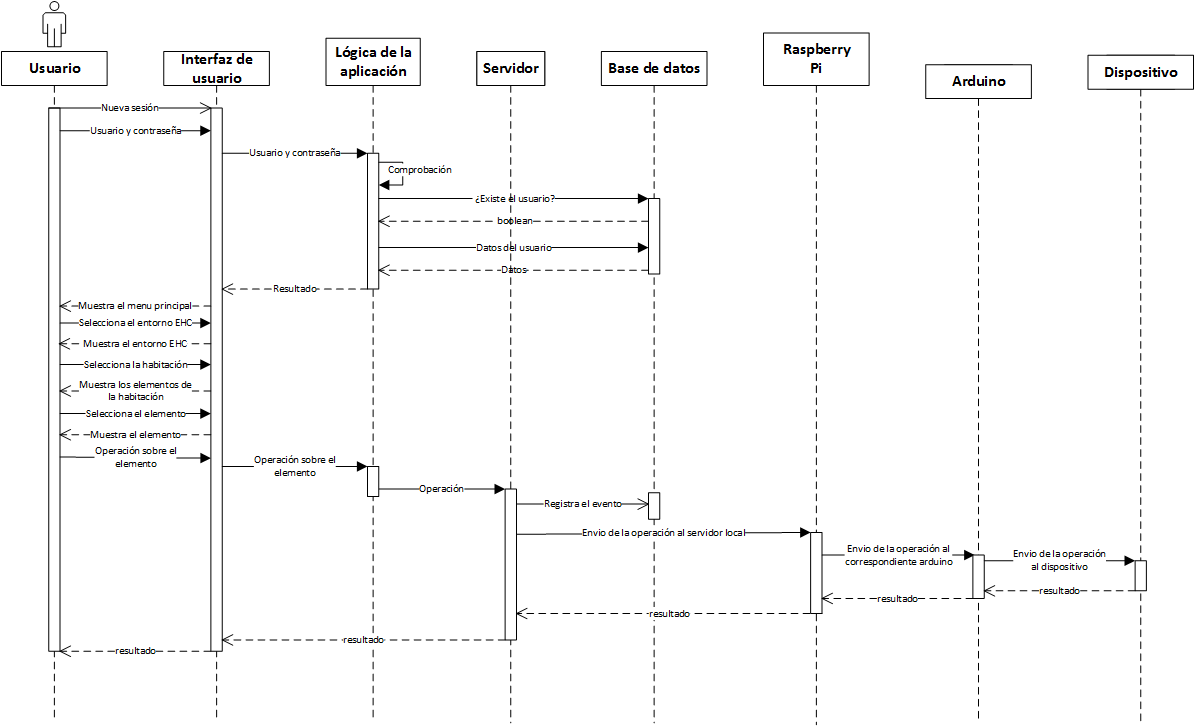
\includegraphics[width=0.9\textwidth]{4.Disenio/Imagenes/DisenioEHC}
	\caption{Diagrama de secuencia de la autentificaci\'on en el sistema y controlar un dispositivo.}
	\label{fig:diagramaSecuencia}
\end{figure}

\begin{figure}
	\centering
	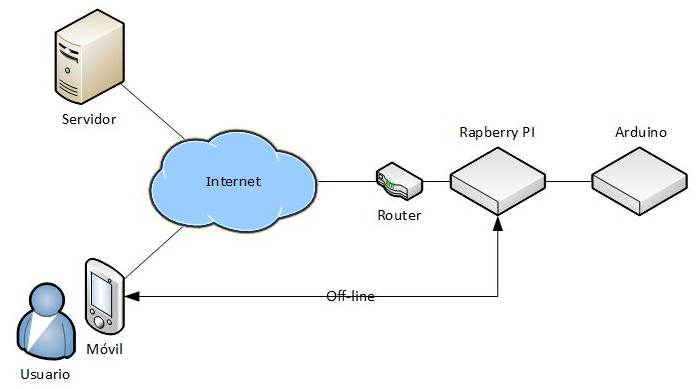
\includegraphics[width=0.8\textwidth]{4.Disenio/Imagenes/arquitectura}
	\caption{Arquitectura del sistema.}
	\label{fig:arquitectura}
\end{figure}


\begin{figure}
	\centering
	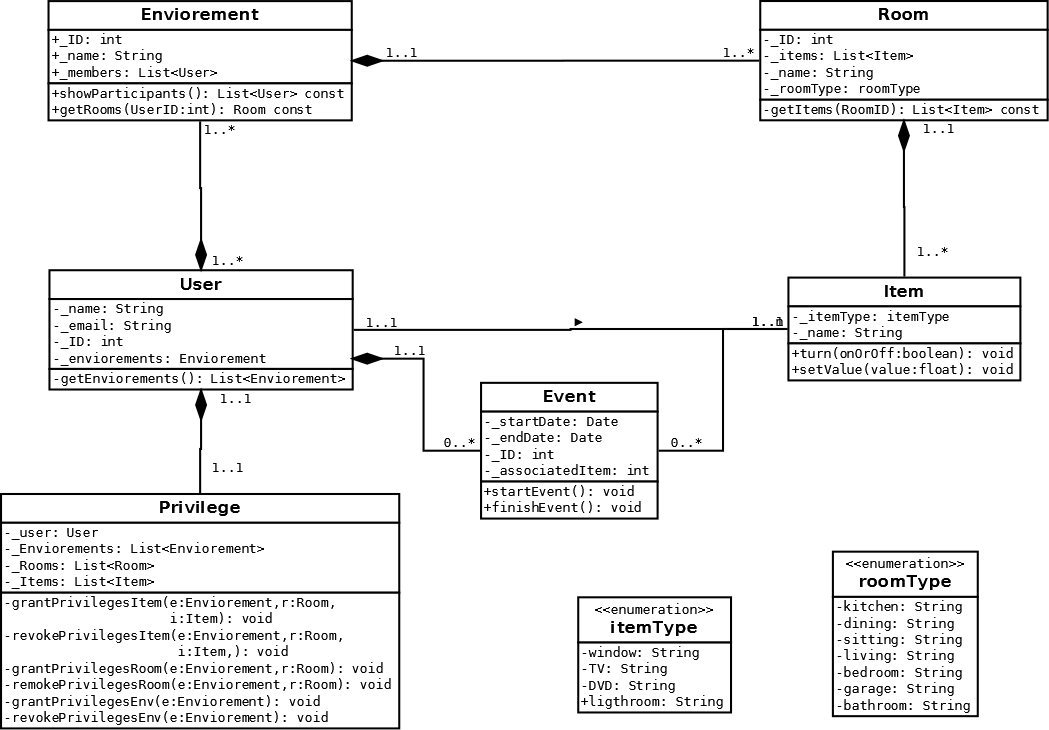
\includegraphics[width=0.8\textwidth]{4.Disenio/Imagenes/diagramaClase}
	\caption{Arquitectura del sistema.}
	\label{fig:diagramaClase}
\end{figure}



(Introducir diagrama de clases, diagrama de comunicacion y diagrama de secuencia)

